\documentclass{beamer}


\usetheme{JuanLesPins}

\usecolortheme{wolverine}


\setbeamercovered{transparent}

\usepackage[T1]{fontenc}
\usepackage[utf8]{inputenc}
\usepackage{url}
\usepackage{multirow}
\usepackage{listings}
\usepackage{graphicx}


\def\BibTeX{\textsc{Bib}\kern-.08em\TeX} 

\newcommand{\footcite}[1]{\footnote{\tiny #1}}
\newcommand{\umlet}{.5}
\newcommand{\emp}[1]{\textit{\alert{#1}}}
\newcommand{\kw}[1]{\mbox{\textbf{#1}}}
\newcommand{\id}[1]{\texttt{#1}}
\newcommand{\stl}{\guillemotleft}
\newcommand{\str}{\guillemotright}

\newcommand{\lsti}{\lstinline[basicstyle=\fontsize{10.5}{12.1}\selectfont]}

\newcommand{\ssection}[1]{
	\section{#1}
	\begin{frame}[fragile=singleslide]\frametitle{}
	\Huge #1
	\end{frame}
}

\newcommand{\ssectionn}[1]{
	\section*{#1}
	\begin{frame}[fragile=singleslide]\frametitle{}
	\Huge #1
	\end{frame}
}

\newenvironment{program}{\begin{beamercolorbox}[rounded=true,shadow=true]{block body}\vspace{-4mm}}{\vspace{-2mm}\end{beamercolorbox}}

\setbeamercolor{fvystup}{fg=white,bg=black}
\newenvironment{vystup}{\begin{beamercolorbox}[rounded=true,shadow=true]{fvystup}}{\end{beamercolorbox}}

\newenvironment{poznamka}{\begin{beamercolorbox}[rounded=true,shadow=false]{block body}}{\end{beamercolorbox}}

\setbeamertemplate{footline}[page number]
{
%\insertpagenumber
%\begin{beamercolorbox}{section in head/foot}
%\vskip2pt\insertnavigation{\paperwidth}\vskip2pt
%\end{beamercolorbox}%
}



\author{Michal Zrutta}
\institute{
	Ústav informatiky, informačných systémov a softvérového inžinierstva\\
	Fakulta informatiky a informačných technológií\\
	Slovenská technická univerzita v Bratislave}

\subtitle{\vspace{3mm} Metódy inžinierskej práce 2023/2024}

\title{Ensuring Data Integrity and Reliability in Big Data
}

\date{\footnotesize 26. november 2023}




\begin{document}

\begin{frame}[fragile=singleslide]
\titlepage
\end{frame}


\begin{frame}[fragile=singleslide]\frametitle{Motivation}
These days data comes too fast and
in an enormous sizes, this requires better understanding of data and processing. The upward trajectory poses challenges in data quality. This study delves into the challenges of data quality assurance in the
realm of Big Data analytic, exploring methodologies to validate diverse
and extensive data-sets. The research focuses on gas consumption in various car models, integrated with AI.
\end{frame}


\begin{frame}[fragile=singleslide]\frametitle{Outline}
\tableofcontents
\end{frame}




\section{What is realm Big Data?}

\begin{frame}[fragile=singleslide]\frametitle{Realm Big Data}
\begin{itemize}
\item Massive amount of information
\item Sources of data
	\begin{itemize}
	\item Social media
	\item Sensors
	\item Online transactions
	\item Multimedia
	\end{itemize}
\item Uniqueness of Big Data
\item Everyday use in industries
\end{itemize}
\end{frame}

\section{Problem Statement}

\begin{frame}[fragile=singleslide]\frametitle{Problem Statement}
\begin{itemize}
\item Wrong data = \emph{change} in overall results
\item How can we ensure data quality?
\begin{itemize}
	\item Data Validity
	\item Data Completeness/Accuracy
	\item Data Consistency
	\end{itemize}
\end{itemize}
\end{frame}

\section{Quality assessment for big data}

\begin{frame}[fragile=singleslide]\frametitle{Quality assessment for big data}
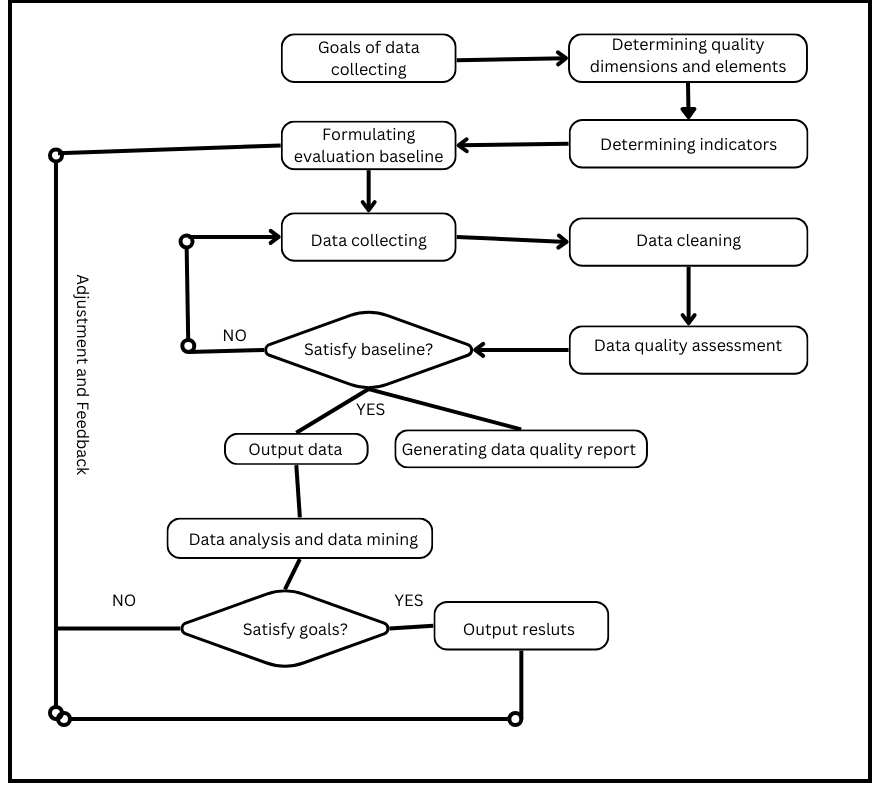
\includegraphics[scale=.32]{Quality assesment process for Big Data.png}\\
{\tiny Quality assessment for big data\ldots}
\end{frame}


\section{Methodology}
\begin{frame}[fragile=singleslide]\frametitle{Methodology}
\begin{itemize}
\item Literature Review
\item Understanding the problem
\item Identification of similar approaches
\item Innovation through Integration
\item Validation through a hierarchical data quality standard
\end{itemize}
\end{frame}

\begin{frame}[fragile=singleslide]\frametitle{Data assessment with AI}
\begin{poznamka}
Example of gas consumption
\end{poznamka}

\begin{itemize}
\item {\textbf{Defining} data collection
goals aligned with strategic objectives}
\item{Implementing a \textbf{user ranking system}}
\item{\textbf{Cleaning} and \textbf{sorting}}
\item Here plays AI great role
\begin{itemize}
	\item AI \textbf{automatically} identifies and corrects mistakes
	\item AI deep understanding of physics
	\item Self-learning mechanism
	\end{itemize}

\end{itemize}
\end{frame}

\begin{frame}[fragile=singleslide]
\frametitle{Data quality indicators}

\resizebox{\textwidth}{!}{%
\begin{tabular}{|l|l|l|}
\hline
\textbf{Dimensions} & \textbf{Elements} & \textbf{Indicators} \\
\hline
\multirow{2}{*}{Availability} & Accessibility & Data access interface provided, easily accessible for public use or purchase \\
\cline{2-3} 
& Timeliness & Data arrival within schedule, regular updates, and timely processing to release \\
\hline
Usability & Credibility & \begin{tabular}[c]{@{}l@{}}Sourced from specialized organizations, regularly audited by experts,\\ and within known/acceptable value range\end{tabular} \\
\hline
\multirow{4}{*}{Reliability} & Accuracy & \begin{tabular}[c]{@{}l@{}}Data provided accurately represent the true state of source information,\\ with unambiguous representation\end{tabular} \\
\cline{2-3} 
& Consistency & Concepts, value domains, and formats remain unchanged after processing \\
\cline{2-3} 
& Integrity & Clear format meeting criteria, consistent structural and content integrity \\
\cline{2-3} 
& Completeness & Deficiency impact on multi-component use, accuracy, and integrity \\
\hline
Relevance & Fitness & \begin{tabular}[c]{@{}l@{}}Data may not fully match the theme but illuminate one aspect,\\ Most retrieved datasets meet user needs and match their retrieval theme\end{tabular} \\
\hline
\begin{tabular}[c]{@{}l@{}}Presentation\\ Quality\end{tabular} & Readability & \begin{tabular}[c]{@{}l@{}}Clear and understandable content, meets user needs, and adheres\\ to specifications in description, classification, and coding\end{tabular} \\
\hline
\end{tabular}
}
\end{frame}


\section{Conclusion}
\begin{frame}[fragile=singleslide]\frametitle{Conclusion}
\begin{itemize}
\item{Effectiveness in ensuring data quality}
\item Reliability and accuracy
\item Importance of a systematic approach
to data quality assurance
\end{itemize}
\end{frame}


\end{document}
 
